\documentclass[../main.tex]{subfiles}

\begin{document}

\subsection{Problem statement}

% {{{ Describe the problem we are trying to solve
More often than not, individuals and organizations face the problem
of visiting a set of destinations in the fastest time possible
in order to carry out an observation.
For example, an operation engineer needs to monitor
a number of reactors and plants during his or her shift.
The need to do so in the shortest time can be due to restrictions on
cost, energy or other limited resources of concern.
This problem is commonly known as the travelling salesman problem
where historically, a salesman had to make a decision in which order
to visit a set of cities exactly once to conduct his trade
in the most time-saving manner.
To achieve that goal, the destinations have to be visited in the order
that is the most efficient in terms of the metric of interest,
and algorithms, such as Dijkstra's, have been successfully used 
to find the shortest path between the cities.

As for the mechanism by which to visit them, 
\textcite{Sha19} deduced that using \glspl{uav}, 
commonly known as drones,
can bring many benefits 
compared to the traditional methods.
Instead of going to the locations in person, installing a \textsc{cctv},
or using satellite technology, a \gls{uav} can provide
high-resolution images or videos without 
having to be installed and maintained at that site
or being restricted to that specific location~\cite{Sha19}.
Moreover, the mobility of the \glspl{uav} is important
in cases where the destinations are actually mobile targets~\cite{Sha19}.
For instance, a marine biologist needs to examine 
the interactions between members of a migrating 
pod of whales whose task neither \textsc{cctv}s 
or satellites are suited for.
If \glspl{uav} are used and such targets move 
in a straight line only,
then the problem can be formulated as 
an optimization problem
and may be solved using mixed-integer programming.
However, if the mobility pattern of the targets is not known,
then such a solution will not work.
This problem, as illustrated in \cref{fig:problem}, 
is what the project at hand intends to solve.
Given some mobile targets' historical locations 
but unknown mobility pattern, 
making a \gls{uav} able to visit them
in the fastest possible time and in turn, 
the most energy-saving way is the goal of this project. 
Particularly, this project aims to demonstrate the 
use of physics simulation in solving it. 
% }}}

% {{{ Figure of the problem
\begin{figure}[tb] 
    \centering
    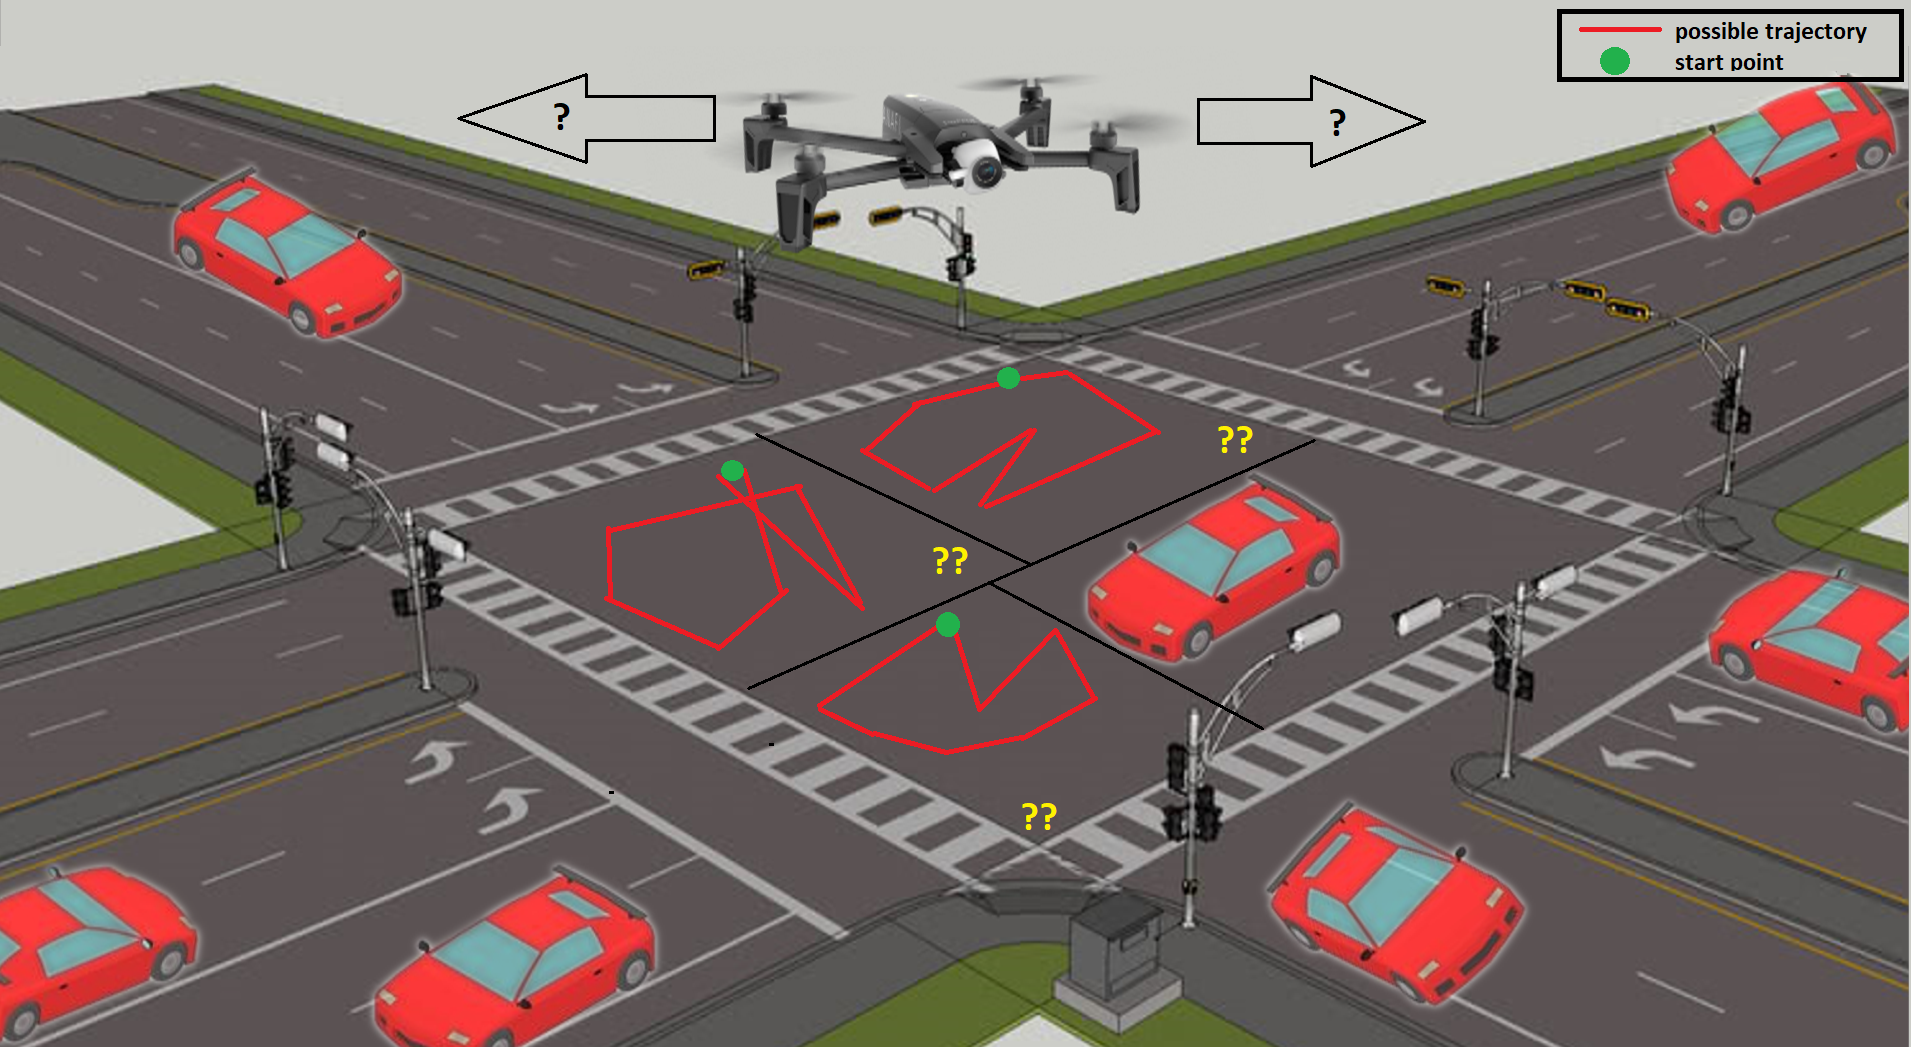
\includegraphics[width=0.9\textwidth]{problem.png} 
    \caption{The \gls{uav} needs to calculate 
    the best trajectory to cover the red cars
    as fast as possible before it runs out of battery.} 
    \label{fig:problem} 
\end{figure}
% }}}

% {{{ Differentiate between technical and non-technical challenges
% {{{{ technical challenges
There are many technical and non-technical challenges
that lie in the path to solving this problem.
Like many other engineering projects,
these challenges have forced us to make trade-offs.
The former category of challenges arises 
from the physical limitations of the drone used to
carry out the observation
and of the computer used to train the \gls{dl} models.
The main technical challenge when working with a drone
is its power supply which is battery powered due to its mobility. 
Other types of power supply such as wireless power transfer
are also possible but infeasible since firstly, it is not the
focus of this project, and secondly, the technology requires 
advanced knowledge which cannot be gained within the set duration.
A similar challenge occurs with the Raspberry Pi attached
to the drone, although its power usage 
is much lower compared to the drone.
The problem with the type of the power supply, in addition to its size, 
is that it directly leads to a host of other technical challenges
such as short flying range and altitude, restricted flying time,
and low allowable payload.
Many of the challenges can be alleviated if the drone model is changed
from the regular \anafi drone to another one such as 
the \anafi \textsc{a}i or the \textsc{dji} 
\textsc{m}atrice 300 \textsc{rtk},
but the cost and shipping logistics as well as
the likely issues with working with a new product
render this solution prohibitive.

In terms of the computer running the \gls{ml} training,
the technical challenge presents itself in terms of 
the accuracy and cost trade-off.
The project involves two \gls{dl} models,
one of which is designed by \textcite{Ged21}.
This \gls{drl} model is used unaltered so 
the computer specifications must minimally be sufficient 
to train it.
The other one is a \gls{dl} model for object detection
used to identify the targets during the training
and its properties are left to our discretion.
For this, 
the depth and width of the model cannot be so big that
a normal data center cannot run although 
being big will improve
the model accuracy. In other words, we need to trade off
the accuracy for the size of the model 
based on the maximum computational resources that we can handle. 
As a result of this, we will have to accept some misses
when the \gls{uav} is detecting the targets during the 
\gls{drl} training, knowing that improving the accuracy 
will not be possible given our limitations.
We estimate that the computer used to develop the \gls{drl} model
should have at least an Intel i5 10th generation or
Ryzen 4000 series \textsc{cpu}, a \textsc{ram} of 8\textsc{gb}, 
and a \textsc{gpu} of at least an \textsc{nvidia} 2000 series
with a \textsc{vram} of 12\textsc{gb}.
% }}}}

% {{{{ non-technical challenges
As for the non-technical challenges, they are caused
by the practical considerations that come
from attempting to solve the problem.
One of the most important of them is cost. 
We have deliberated that
the resulting price for the stakeholders or clients
should not exceed \textsc{qar}~6000. 
This means that the fixed and variable costs of this project
come from procuring the \anafi drone, the Raspberry Pi and other
components in the system, 
and wages for designing and training the model  
should be around \textsc{qar}~4000 to make a 30\% target profit.
The second non-technical challenge that we are required to consider
is the logistics of procuring the materials and devices above.
The \anafi drone, its spare parts and special Raspberry Pi
components required in the solution are only available abroad.
Not only do they cost more due to the additional shipping charge,
but they are also limited in number 
and take more time to arrive, which can delay 
and disrupt the progress.
Finally, since using the Parrot \anafi drone in \gls{drl}
is a niche area of research and new on the market,
it is challenging to find learning resources for the tools
that are used to program both technologies
and the community to find support from is markedly small.
% }}}}
% }}}

\subsection{Project significance}

% {{{ Project importance
Completing this project, which will provide the solution
to using a simulation and \gls{drl} in making an intelligent drone 
that is able to visit mobile targets in the shortest time,
holds lasting and critical importance 
in the local and global societies.
First of all, the \gls{uav} combines the best features
from \textsc{cctv}s and satellites.
Using \glspl{uav} gives the benefit of high resolution images
for the purposes of surveillance and monitoring
similar to \textsc{cctv} cameras 
without the restriction in movement~\cite{Sha19}.
At the same time, it allows for large-scale monitoring 
usually done exclusively using satellites 
without its low accuracy~\cite{Sha19}.
Second of all, target visitation done by a \gls{uav}
is faster because it has a higher degree of freedom
compared to terrestrial vehicles and
it flies at a higher altitude 
making it more able to avoid 
many of the surrounding obstacles.
Being another major aspect of the project, \gls{drl}
allows the \gls{uav} to generalize better
making it perform more robustly
in an unknown environment
and with unknown targets mobility patterns.
Finally, using physics simulation will make the product 
more accurate since it considers 
environmental noise and
the kinematics and dynamics of the \gls{uav} more accurately.
Consequently, the training of the \gls{drl} model 
using the simulation will be improved 
and the performance will be better
compared to using a merely mathematical simulation.
% }}}

% {{{{ Describe how can stakeholders use the project,
% ## its uses/applications,
% ## impacts if the design problem was not solved,
% ## and benefits of the project in Qatar and the region.
Based on the project's significance, we have identified 
its stakeholders to be 
those companies, institutions and organizations which
have certain fixed or mobile subjects of interest 
that they want to monitor, capture or track.
By using our product,
they will be able to make these tasks faster or,
better yet, possible.
Applications range from criminal tracking 
to wildlife monitoring,
and from security surveillance
to last-mile delivery.
The absence of this project will mean that
the aforementioned tasks will remain
time-consuming, tedious and expensive
while some will remain infeasible
causing the stakeholders to be deprived of ample growth opportunities.
In some instances, the difference between using 
and not using an intelligent \gls{uav} 
\gls{drl}-trained on mobile target visitation
will be a matter of life-and-death
such as in the search-and-rescue field.
Moreover, Qatar stands to benefit the most from this project 
considering the \textsc{fifa} 2022 it will be hosting
and its rapidly transforming economy and population.
For example, the use of drones can help manage 
the \textsc{fifa} World Cup 
and the increase in population through better monitoring 
of traffic and people, whose data can contribute
to better studies in those sectors.
In addition, the Covid 19 has made online shopping
the number one choice for 
the majority of people to buy goods in Qatar~\cite{Has20}.
The success of this project can help in delivering
the goods to intended destinations with minimum delay,
thus contributing to a healthy economy.
% }}}

% {{{ Why do you want to do this project? 
% # What got you interested in it? 
% # And how this project will help you further your career goals?
The project's significance even extends to the authors
on a personal and individual level.
The prime evidence that has attracted the authors to invest
their energy and time in this project is
the increasing number of giant companies like Amazon, Alphabet
and Microsoft experimenting with and profiting from \glspl{uav}
to improve their operations~\cite{Jun17}.
Target visitation is an important subtask of these among others.
Therefore, we believe there is a huge value
in this project and upon the successful completion of it,
there will be many doors opening up to us in terms of
career opportunities because 
this technology is in high demand yet, 
people with the right competency
are scarce.
Besides the jobs that are directly related to the project,
there are other fields that will appreciate the knowledge
and skills that we will gain from the methodological processes 
of designing the simulation,
training the \gls{drl} models and testing them in the real world.
These include robotics, machine learning, and 
network security.
% }}}

% # Possibly cite relevant references that discuss 
% # the importance of our project

\subsection{Project objectives}\label{sec:objectives}

% {{{ Express clear specific objectives
The \gls{uav} enjoys the benefits of \textsc{cctv}s and satellites
in surveillance and monitoring without their drawbacks.
Therefore, it has the potential to replace these
traditional technologies in many applications, 
most of which involve mobile target visitation. 
Although there exist a few studies 
that have investigated it in terms of \gls{drl}-trained
\gls{uav},
none of them thus far have attempted to
integrate a physics simulator in the training
and demonstrate the product in the real world.
The aim of this project is hence to create a process 
by which a physics simulator is used to train 
a \gls{drl} model that will later be used
to make a \gls{uav} accurately accomplish a
mobile target visitation task.
The project's detailed objectives are as follows:

\begin{enumerate}
    \item \label{obj:drl} Develop a \gls{rl} 
        training framework,
        which utilizes a physics simulator, 
        that implements the \gls{drl} model 
        published in the \textcite{Ged21} paper.
    \item \label{obj:hardware} Construct a 
        physical \gls{uav} system 
        using the \anafi drone and 
        Raspberry Pi that together is able to execute
        a target visitation mission autonomously.
    \item \label{obj:demo} Evaluate the trained 
        model using this system
        and several targets in a physical environment.
\end{enumerate}
% }}}

% {{{ Deliverables and desired results
To demonstrate the objectives, there will be a number 
of deliverables that we will produce.
Firstly, we will present a detailed report 
that will elaborate on our aim, objectives, 
literature review, methodology,
solution and the market value of the project.
Secondly, we will output a trained \gls{drl} model for 
the target visitation task of a specific
mobility pattern.
Finally, we will build a \gls{uav} system
consisting of the \anafi drone as well as a Raspberry Pi
that will contain the model and instruct
the \anafi drone throughout the mission.
Based on the deliverables, the desired result is that
given the same mobility pattern for 
the moving targets as the one in the \gls{drl} training,
the \gls{uav} should be able to fly to locations it has learned
and this will allow it to capture the maximum targets. 
In other words, it should anticipate that these 
locations are those it can reach
the quickest and also where most targets will gather.
In doing so, it will prove that it can accomplish 
the mobile target visitation task in an uncertain environment
for an unknown target mobility pattern
as long as the target movements can be simulated.
% }}}

\end{document}
